\documentclass[../thesis.tex]{subfiles}
\externaldocument[I-]{./basics}
\graphicspath{{\subfix{../resources/}}}
\begin{document}

\chapter{Discussion}\label{chapter:discuss}

\section{Features in multiple groups} \label{sec:discussion:mutually_exclusive_group_size}

% Nur aus Neugier, ohne eine Lösung: Wie könnte man das Problem angehen?
% Bräuchte man hier einfach mehr MEssungen/Gruppierungen? Ist ein Punktfür die Diskussion
To allow bigger group sizes than the smallest group of mutually exclusive features,
we let mutually exclusive features to be in multiple groups in a round of grouping, which diverts 
from the setup of group sampling described by \citeauthor{saltelli2008global}.
Groups of two mutually exclusive features are not uncommon and would limit the
number of groups to two groups. This would make learning the influence of features
in bigger systems with group sampling more difficult.
If, for example, a feature that is in more than one group is an influential feature,
it would effectively render the groups the feature is in, as one group.
All the groups would get assigned the influence of the influential feature.
But even if the features, which are in multiple groups, are non-influential features,
it causes some problems. Because it is enabled in more groups than
other features, it is more likely to repeatedly share a group with an influential feature
and make it look more influential than it actually is.
Both problems, if the feature is influential and if it is not, could be avoided if
the feature is not mandatory. It could simply be enabled just once per round of groupings.
If the feature is mandatory, a way to mitigate the problem is by increasing the amount
groupings made. More groupings and measurements made should make it easier to
determine the influence of the feature in multiple groups.


\section{Identifying influential features} \label{sec:discussion:mutually_exclusive_group_size}

We have seen the performance influence model created with group sampling does not perform as well
as a more straightforward approach such as random or distance based sampling does. If the goal is to predict
the performance of a system, group sampling showed to be less effective than, for instance, random sampling with linear regression.
In \autoref{sec:evaluation:scalability}, we looked at the coefficients of the created model.
While the group sampling algorithm was able to determine the influential features, the
estimations of the created model were unreliable. Nonetheless, the information the group sampling
algorithm gives us can be useful. With the identification of an influential feature, we can, for example, make assumptions
about inefficient parts of the system.
In \autoref{fig:discussion:coefficients} and \autoref{fig:discussion:coefficients_box} we can see that group sampling was able to identify
the influential feature with fewer samples than distance based sampling with a linear regression
on our synthetic dataset. This might be used to screen an existing feature model for further analysis.

\begin{figure}[h]
      \begin{center}
            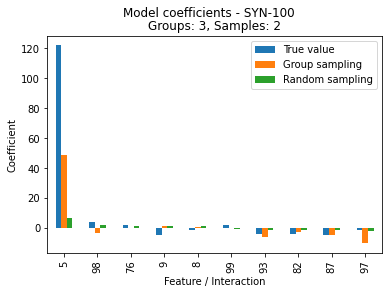
\includegraphics[width=0.5\textwidth]{graphs/syn-100-model-coefficient.png}
      \end{center}
      \caption[Model coefficients - SYN-100 dataset]{
            Model coefficients with 3 groups and 2 samples
      }\label{fig:discussion:coefficients}
\end{figure}





\begin{figure}[h]
      \begin{center}
            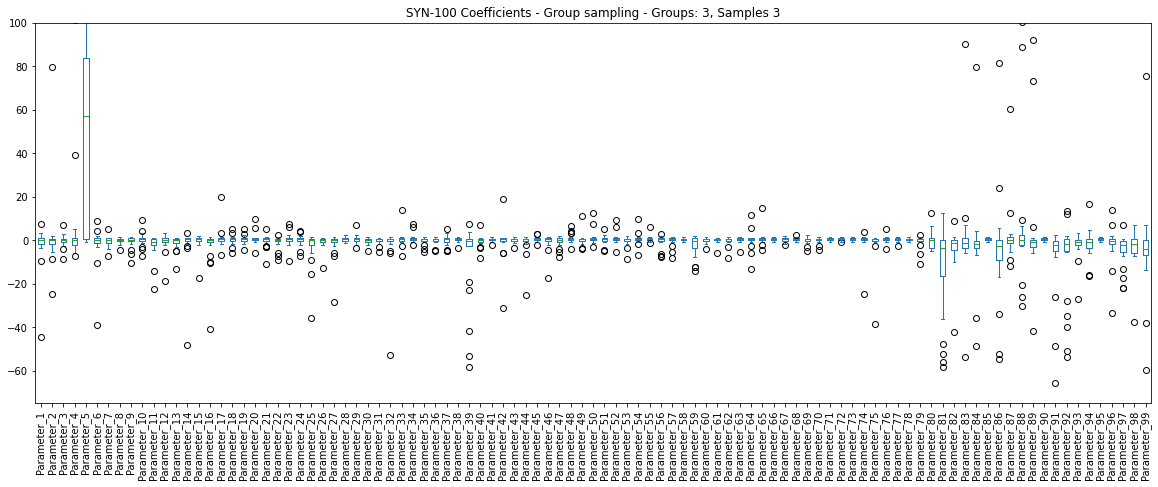
\includegraphics[width=1\textwidth]{graphs/syn-100-gs-box.png}
            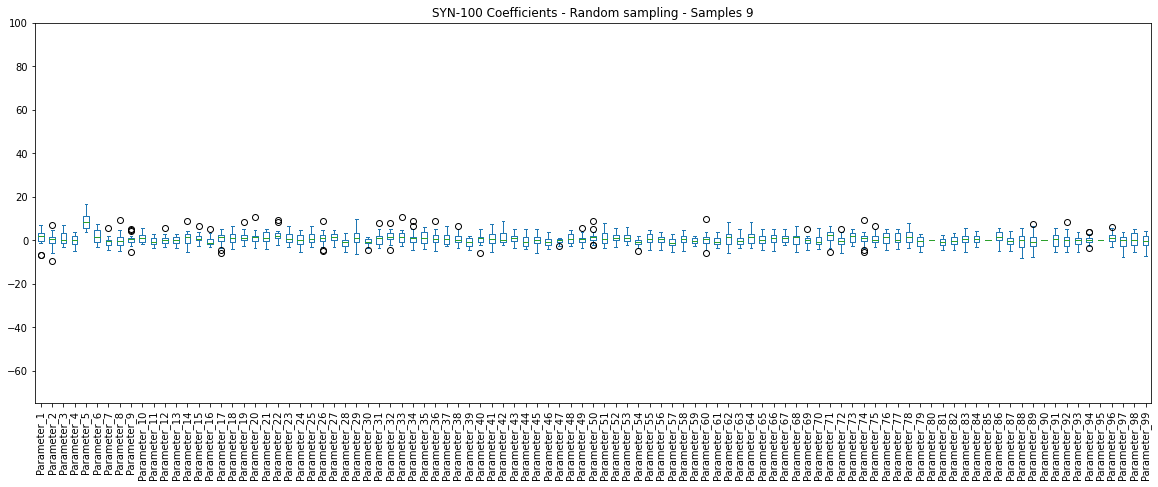
\includegraphics[width=1\textwidth]{graphs/syn-100-random-box.png}
      \end{center}
      \caption[Model coefficients - SYN-100 dataset - Box plot]{
            Model coefficients with 3 groups and 3 samples on the SYN-100 Dataset
      }\label{fig:discussion:coefficients_box}
\end{figure}

\begin{figure}[h]
      \begin{center}
            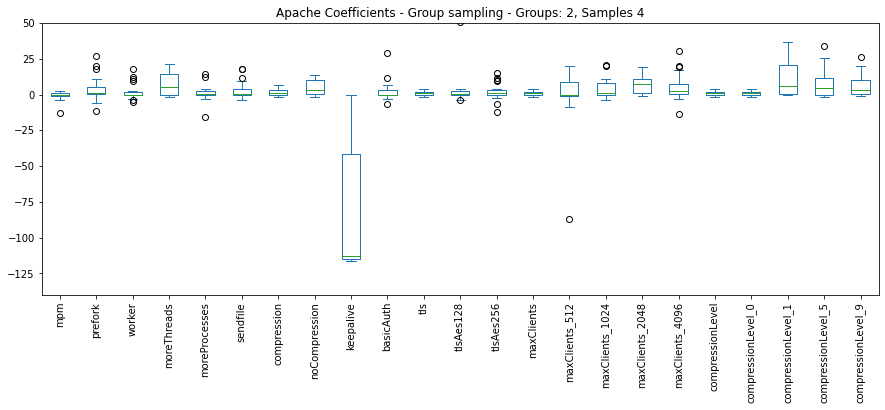
\includegraphics[width=1\textwidth]{graphs/apache-gs-box.png}
            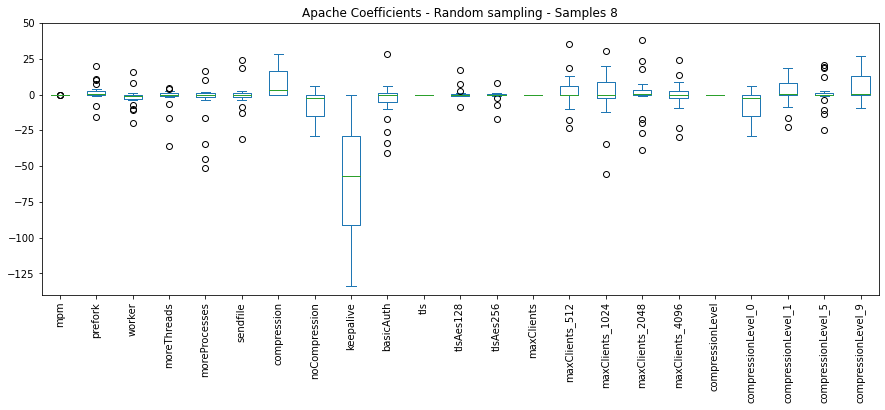
\includegraphics[width=1\textwidth]{graphs/apache-random-box.png}
      \end{center}
      \caption[Model coefficients - Apache dataset - Box plot]{
            Model coefficients with 2 groups and 4 samples on the Apache dataset
      }\label{fig:discussion:coefficients_box_apache}
\end{figure}


\section{Influence estimations of non-influential features}\label{sec:discussion:estimate}

During our tests, we noticed that a major reason for the unreliability of our model is the inaccurate
estimation of the influence of non-influential features. The coefficients for the model created
by our approach to group sampling had a relatively high variance on non-influential features
and often did not improve significantly with more samples. In \autoref{fig:discussion:coefficients}
we can see a lot of outliers in the estimated influence values. 
We can explain the positive outliers by features sharing a group with an influential feature too many times.
Especially the outliers in mutually exclusive groups, since they are in more groups than independent features.
The negative outliers can to some degree be explained by how we create the model. 
If we look at \autoref{eq:group_sampling:intercept} we determine $f_0$ by the average of all influence values.
With a few groups, the average of all influence values is significantly affected by 
the influential feature. If we assume we have a dataset with only independent features and apply a group sampling
approach as we described with only two groups, in each round of grouping, half the features get assigned
the value of the influential feature, resulting in an average of all influence values between the baseline performance
and the influence of the influential feature. As \autoref{eq:group_sampling:coefficient} shows, the value of $f_n$ 
is dependent on the determined baseline performance $f_0$, making $f_n$ inaccurate if $f_0$ is inaccurate.  
Especially features, which do not share a group with the influential feature are affected leading to 
a large error in the opposite direction of the influence of the influential feature.
With more groups, this effect reduces, but it leads to significant problems with smaller group sizes.


\end{document}